\subsection{Active Armrest}
\begin{figure}[h]
\centering
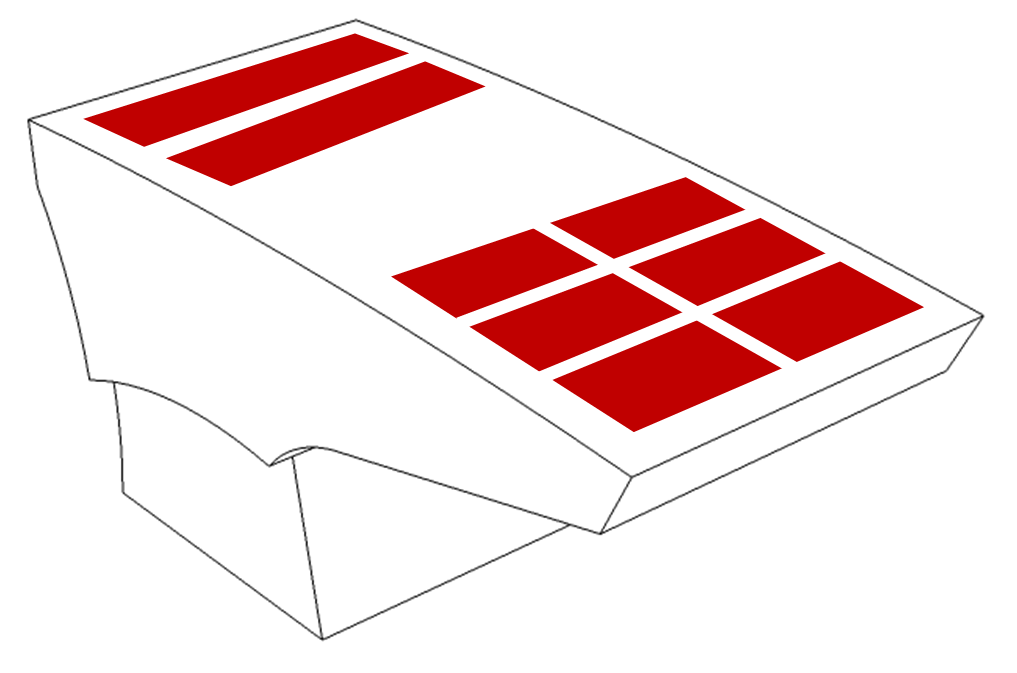
\includegraphics[width=0.4\textwidth]{images/active_armrest}
\caption{Active armrest sketch - six electrodes for finger gesture detection in front, two for arm detection in back}
\label{fig:armrest_sketch}
\end{figure}
Touch screens are by now one of the most ubiquitously used interaction method in HMI with billions of finger-controlled smartphones being in use [9]. This trend is also apparent in vehicles, with touch screens and touch pads becoming more common. The Tesla Model S provides a large area touch screen that completely replaces conventional button-based interfaces. BMW augmented their iDrive control system with a touchpad that is able to recognize finger gestures. However, touchscreens have been identified as potentially distracting for the driver [12] and systems like iDrive rely on mechanical control systems that protrude from the other features of the car interior. Capacitive touch sensing is the most common technology for creating touchscreens [2]. A variety is capacitive proximity sensing that enables to detect the presence of conductive objects, such as the human hand over a distance [14]. It can be used to create gesture input devices that recognize free-air hand or finger movements [4]. As it is based on measuring the electric field it can be applied below any non-conductive material, e.g. plastic, wood, or leather that are commonly used in car interiors. Thus, we can create interactive surfaces and interactive zones in free-air that sense the movement of the hand, yet are completely integrated into a car environment. 
A suitable area for creating an interactive zone is the armrest, as it is the intended resting position in the first place. However, this creates an additional challenge. As the majority of interactions between arm and armrest are not intended to control aspects of the car system, we need concepts to infer the intention of the driver to interact with the car. We propose two different methods that utilize the capability to detect the presence and distance of the arm from the surface. The first option enables interaction only when the arm is raised and fingers are touching the interactive area in front of the armrest. The second option assumes that the arm is resting on the surface and the fingers are performing small gestures above the interactive area in the front. 
To test the validity of the invisible interactive areas and the two interaction concepts, we have created the Active Armrest, a prototype comprised of an aftermarket armrest with an integrated heterogeneous array of eight capacitive proximity sensors - two using large electrodes for detecting arm proximity and orientation and six using small electrodes to create an interaction area in front of the armrest. We have adapted methods to classify both free-air and touch gestures for capacitive proximity sensors using a SVM classification method and created a demonstration application that mimics typical multimedia functions in a car. We have performed an evaluation of the classification precision and a usability test of both methods in a study with ten participants.
2.	RELATED WORK
The list of research into automotive interfaces is extensive. Alpern and Minardo presented a study on different forms of gesture interaction within a car, performed by the right hand while the left stays on the wheel [1]. The effects of the interaction were displayed on a HUD. They found that gestural interfaces in their setup were preferred to traditional interfaces for secondary tasks, if the visual feedback was appropriately designed.

Bach et al. compared three different interaction techniques in cars and their effects on driving performance and visual distraction. They found that interaction on touch screens is fastest, but most distracting and that gestural interaction, while slower, does not lead to an increase in interaction errors [8].
Regarding large touchscreens, e.g. used in the Tesla Model S, Rümelin and Butz explore different interfaces, including adding a knob as physical element [11]. They discovered that there was an advantage in learnability and task completion time for all direct touch interfaces, as opposed to remotely controlled systems and that driving performance was not affected negatively.
Döring et al. integrated a multi-touch system into a common steering wheel to enable distraction free control of comfort functions in a car [6]. The system also allows creating different visual interfaces in the steering wheel. Their findings include a significantly reduced visual load as opposed to center console touch navigation and button controlled radio.
Burnett et al. compared rotary controls, touchpads and touchscreens for their performance in different tasks [5]. They found that rotary controls performed the worst and that preference for touchscreen or touchpad is depending on the task, with the first having an advantage in more complex menus and the latter being preferred in tasks that can be completed using simple commands.
Pfleging et al. combined speech input and gestures performed on a tablet integrated into the steering wheel [10]. They showed that this approach has similar distraction compared to traditional interfaces, while providing a higher degree of flexibility.


\subsubsection{Evaluation}
\begin{figure}[h]
\centering
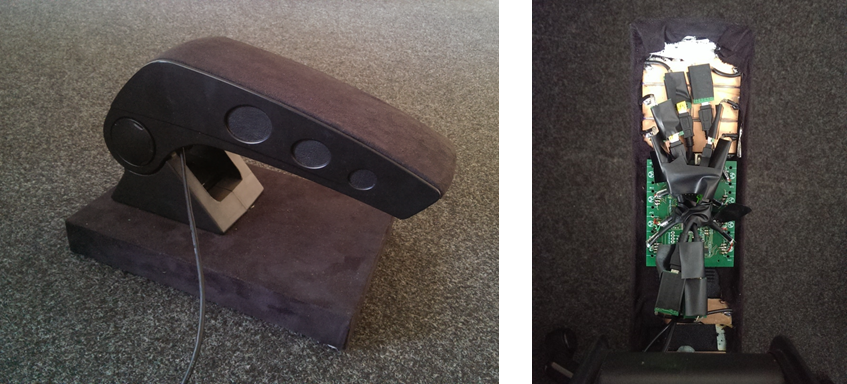
\includegraphics[width=0.8\textwidth]{images/armrest_proto}
\caption{Active Armrest prototype, left - outside view, right - detail view of electronics}
\label{fig:armrest_proto}
\end{figure}
%Figure 26 Active Armrest prototype, left - outside view, right - detail view of electronics
In order to evaluate the Active Armrest we have built the prototype shown in Figure \ref{fig:armrest_dataproc}. An aftermarket armrest was equipped with an OpenCapSense toolkit. The demonstration application is based on the SenseKit debug software supplied with the toolkit. As of now there is a simple USB connection to a nearby PC.
\begin{figure}[h]
\centering
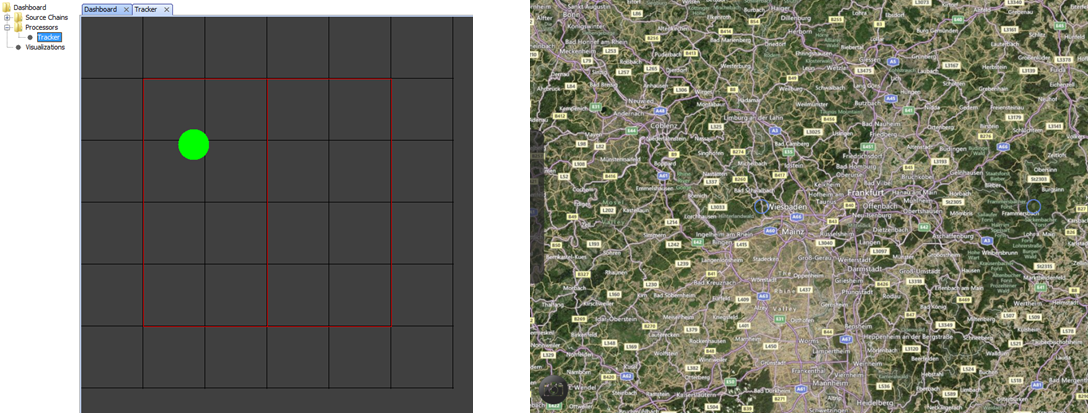
\includegraphics[width=0.6\textwidth]{images/armrest_eval}
\caption{Active Armrest demo software, left - finger tracker, right - OSM based navigation application}
\label{fig:armrest_eval}
\end{figure}
%Figure 27 Active Armrest demo software, left - finger tracker, right - OSM based navigation application
Figure \ref{fig:armrest_eval} shows a screenshot of the finger tracking application on the left, with a two-finger touch registered on the upper left part of the touch area. It is interfaced with a TUIO \cite{kaltenbrunner2005tuio} based maps application using OpenStreetMap \cite{haklay2008openstreetmap} data. The map is moved around using simple swipe movements of the finger that are directly associated to pan-features of the demonstration application. Zooming is activated by two-finger hold gestures on the upper or lower part of the touch area. We have used public displays of this prototype to get an idea of how easily unaffiliated persons learn to use the system. While the majority agreed on the potential of the application, there have been some reservations regarding the current gesture set, particularly that a closer relationship to smartphone touch screen gestures would be welcome.

\begin{minipage}{\linewidth}
\centering
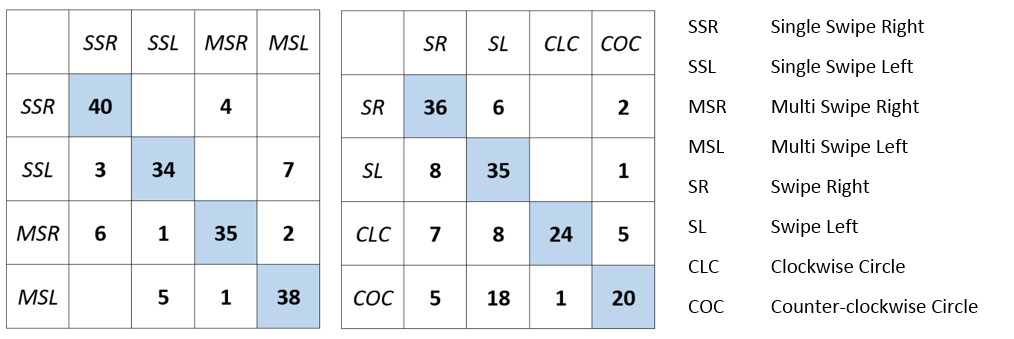
\includegraphics[width=0.7\textwidth]{images/armrest_eval_confustion}
\captionof{figure}{Confusion matrices of recognized gestures for touch interaction (left) and free-air interaction (right)}
\label{fig:armrest_eval_confustion}
\end{minipage}

We performed a study with 11 participants investigating three different aspects - the detection rate of the gesture recognition system, differences in interaction speed between the two methods and getting a general feedback on the usability of our system. After a short introduction the participants were asked to perform each gesture 4 times for both sets in alternating starting order. The results are shown in Figure \ref{fig:armrest_eval_confustion}. The touch interaction performed reasonably with a detection rate between $79.5\%$ and $90.9\%$ for each gesture. The detection rates of the free-air interaction were considerably lower, ranging from $45.5\%$ for counter-clockwise circles to $81.8\%$ for swipes to the right. The main issue is distinguishing between single and multi-touches. A personalized threshold that is calibrated to the user might alleviate this issue in future iterations. The interaction zone above the finger area is limited to a range of about 15 cm. While performing the circular gestures the participants often left this area, leading to misattribution to swipe gestures.
In the second part of the evaluation the participants had to perform a task in the presented demonstration application - selecting and playing back a certain music file. We calculated the time required to perform the task. The average time for free-air gestures ($\mu=125.67s, \sigma=95.12s$) was considerably higher than the average task completion time for touch gestures ($\mu=34.26s, \sigma=28.61s$). It is noticeable that there is a very high deviation of the different runs, while the touch gestures fare better in general. While many users were able to quickly perform the task, others had a high number of errors and required several minutes. We can assume that a certain amount of training can reduce the required time. A trained user not participating in the study required 11s for the touch gestures and 18s for the free air gestures.
Finally, we asked the participants to fill a general questionnaire on their experience with the Active Armrest comprised of a number of Likert-scale (1-10) questions. There was a strong preference for the touch gestures, in line with the results of the interaction time and gesture recognition study (1=touch gestures, $\mu=1.72, \sigma=0.84$). Most participants could imagine using the system for a longer period of time in their cars (10=strong agree, $\mu=8.00, \sigma=2.00$) and considered the device intuitive to use (10=strong agree, $\mu=8.36, \sigma=1.67$) and is an interesting interaction device (10=strong agree, $\mu=8.63, \sigma=1.26$). The touch interaction pattern was considered easier to use (10=very easy, $\mu=8.00, \sigma=2.45$) than the free-air interaction (10=very easy, $\mu=3.64, \sigma=2.68$). The opinions on the device precision were mixed (10=very precise $\mu=7.27, \sigma=2.43$).

